$n \in \mathbb{N}; m \in \mathbb{N};\ \binom{n}{k}$  gelesen ''n über m'' $n < m \Rightarrow \binom{n}{m} = 0$ $n \geq m \Rightarrow \binom{n}{0} = 1,\ \binom{n}{1} = n,\ \binom{n}{n}$
$$\binom{n}{m} = \frac{n(n-1) \dots \cdot (n-m-1)}{1\cdot 2\cdot3 \dots m} = \frac{n!}{m!(n-m)!}$$
$$\binom{n}{m}=\binom{n}{n-m}$$ Jeweils $m$ viele Faktoren, da sich der Rest wegkürzt.
z.b:
$$\binom{4}{2} = \frac{4 \cdot 3 \cdot \cancel{2 \cdot 1}}{2 \cdot 1 \cdot \cancel{2 \cdot 1}} = \frac{12}{2} = 6;\ \binom{5}{3} = \binom{5}{2} = \frac{5 \cdot 4 \cdot  \cancel{3 \cdot 2 \cdot 1}}{2 \cdot 1 \cdot \cancel{3 \cdot 2 \cdot 1}} = 10$$
Kombinatorische Bedeutung: Anzahl der m-elementigen Teilmengen einer n-elementigen Menge
$$\binom{n}{m}+\binom{n}{m+1}=\binom{n+1}{m+1}$$
\begin{alignat*}{1}
    \binom{n}{m}+\binom{n}{m+1} & =\frac{n!}{m!(n-m)!}+\frac{n!}{(m+1)!(n-m-1)!}=\frac{n!(m+1)+n!(n-m)}{(m+1)!(n-m)!} \\
    & =\frac{(n+1)!}{(m+1)!((n+1)-(m+1))!}
\end{alignat*}
Pascalsches Dreieck: \\
\begin{tabularx}{\linewidth}{@{}*2{>{\centering\arraybackslash}X}}
    \begin{tikzpicture}
        \node (11) at (0, 0) {1};
        \node (21) at (-0.5, -0.5) {1};
        \node (22) at (0.5, -0.5) {1};
        \node (31) at (-1, -1) {1};
        \node (32) at (0, -1) {2};
        \node (33) at (1, -1) {1};
        \node (41) at (-1.5, -1.5) {1};
        \node (42) at (-0.5, -1.5) {3};
        \node (43) at (0.5, -1.5) {3};
        \node (44) at (1.5, -1.5) {1};
        \node (51) at (-2, -2) {1};
        \node (52) at (-1, -2) {4};
        \node (53) at (0, -2) {6};
        \node (54) at (1, -2) {4};
        \node (55) at (2, -2) {1};
        \node (61) at (-2.5, -2.5) {1};
        \node (62) at (-1.5, -2.5) {5};
        \node (63) at (-0.5, -2.5) {10};
        \node (64) at (0.5, -2.5) {10};
        \node (65) at (1.5, -2.5) {5};
        \node (66) at (2.5, -2.5) {1};
    \end{tikzpicture} &
    \begin{tikzpicture}
        \node (11) at (0, 0) {$\binom{0}{0}$};
        \node (21) at (-0.5, -0.5) {$\binom{1}{0}$};
        \node (22) at (0.5, -0.5) {$\binom{1}{1}$};
        \node (31) at (-1, -1) {$\binom{2}{0}$};
        \node (32) at (0, -1) {$\binom{2}{1}$};
        \node (33) at (1, -1) {$\binom{2}{2}$};
        \node (41) at (-1.5, -1.5) {$\binom{3}{0}$};
        \node (42) at (-0.5, -1.5) {$\binom{3}{1}$};
        \node (43) at (0.5, -1.5) {$\binom{3}{2}$};
        \node (44) at (1.5, -1.5) {$\binom{3}{3}$};
        \node (51) at (-2, -2) {$\binom{4}{0}$};
        \node (52) at (-1, -2) {$\binom{4}{1}$};
        \node (53) at (0, -2) {$\binom{4}{2}$};
        \node (54) at (1, -2) {$\binom{4}{3}$};
        \node (55) at (2, -2) {$\binom{4}{5}$};
        \node (61) at (-2.5, -2.5) {$\binom{5}{0}$};
        \node (62) at (-1.5, -2.5) {$\binom{5}{1}$};
        \node (63) at (-0.5, -2.5) {$\binom{5}{2}$};
        \node (64) at (0.5, -2.5) {$\binom{5}{3}$};
        \node (65) at (1.5, -2.5) {$\binom{5}{4}$};
        \node (66) at (2.5, -2.5) {$\binom{5}{5}$};
    \end{tikzpicture}
\end{tabularx}
$$\sum\limits_{k=1}^n \binom{k}{m} = \binom{1}{m}+\binom{2}{m}+ \dots + \binom{m}{n}+\binom{m}{m}+\binom{m+1}{m}+\dots+\binom{n}{m}=\binom{n+1}{m+1}$$
$$\sum\limits_{k=1}^n\binom{k}{1} = \frac{n(n+1)}{2}$$
Binomialsatz
$$(a+n)^n=\sum\limits_{m=0}^n\binom{n}{m}a^{n-m}b^m=a^n+\binom{n}{1}a^{n-1}b+\binom{n}{2}a^{n-2}b^2+\dots + \binom{n}{n-1}ab^{n-1}+b^n$$